% Challenge report - Deep Learning (SRH). IEEE conference format, 2-4 pages incl. figures and tables
% (references do not count). Compile: pdflatex report, bibtex report, pdflatex report, pdflatex report
% - or upload the whole folder to Overleaf (New Project -> Upload Project).
% Every number below comes from results/summary.csv, results/test/*.json and
% results/figures/ of the Git repository (tag v1.0-final); none is typed from memory.
\documentclass[conference]{IEEEtran}
\usepackage{graphicx}
\usepackage{booktabs}
\usepackage{amsmath}
\usepackage{url}

\begin{document}

\title{Logit Adjustment Meets Transfer Learning:\\ Balanced Skin-Lesion Classification on DermaMNIST}

\author{\IEEEauthorblockN{Ossai Ron}
\IEEEauthorblockA{SRH University}
\and
\IEEEauthorblockN{Ifroon Griffin}
\IEEEauthorblockA{SRH University}
\and
\IEEEauthorblockN{Faraz Saedi}
\IEEEauthorblockA{SRH University}
\and
\IEEEauthorblockN{\textit{Team: Am besten}}}

\maketitle

\begin{abstract}
We classify 28$\times$28 dermatoscopy images of DermaMNIST into seven lesion types, two thirds of which are
harmless moles, and optimise balanced accuracy. Starting from the starter CNN (validation balanced accuracy
0.461~$\pm$~0.011 over three seeds), we tested ten single changes, each with three seeds and a 95\,\% paired
bootstrap interval against the baseline. Correcting the class imbalance helped most: a logit-adjusted loss
raised validation balanced accuracy to 0.532~$\pm$~0.031. Combined with an ImageNet-pretrained ResNet-18 on
upsampled inputs and flip/rotation augmentation, it reached 0.590~$\pm$~0.017, and an ensemble of the three
seed models reached 0.609. On the official test set, evaluated once, this model scores 0.632 balanced
accuracy against 0.448 for the baseline ensemble ($\Delta$~+0.184, 95\,\% CI [+0.136, +0.232]). The gain
comes from finding rare classes, at the price of more moles being called something else.
\end{abstract}

\section{Introduction}
A useful skin-lesion classifier must recognise every lesion type, not only the most common one. In DermaMNIST 67\,\% of the training images are melanocytic nevi, so a model that always
answers ``nevus'' reaches 67\,\% accuracy but finds no melanoma; its balanced accuracy (mean sensitivity over
the seven classes) is 1/7. Balanced accuracy weights every class equally, including rare benign ones such as
dermatofibroma, so we select and report every model by it.
Our contributions: (i) a controlled comparison of ten single changes to the starter baseline, each with three
seeds and a bootstrap interval; (ii) a stack of the helpful changes, chosen on validation data only;
(iii) evidence that the imbalance correction and the pretrained network help each other.

\section{Data}
DermaMNIST~\cite{medmnistv2} contains the HAM10000 dermatoscopy images~\cite{tschandl2018ham} resized to
28$\times$28 RGB, with the official split of 7\,007 training, 1\,003 validation and 2\,005 test images
(Table~\ref{tab:data}). The imbalance is 59:1 between nevi (4\,693) and dermatofibroma (80); the validation set
holds only 12 dermatofibroma and 14 vascular images, so their sensitivities change by 7--8 points per image.
Images are scaled to [0,1] and normalised with the starter's per-channel mean (0.7631, 0.5381, 0.5614) and
std (0.1366, 0.1543, 0.1692); augmentation, where used, is applied to training images only.
The 28$\times$28 resolution removes fine texture and borders, and HAM10000 can contain several images of the
same lesion; we use the official splits as given and treat this as a limitation.

\begin{table}[t]
\caption{Images per class and split}
\label{tab:data}
\centering
\begin{tabular}{llrrr}
\toprule
label & class & train & val & test \\
\midrule
akiec & actinic keratoses$^{\dagger}$ & 228 & 33 & 66 \\
bcc & basal cell carcinoma & 359 & 52 & 103 \\
bkl & benign keratosis-like lesions & 769 & 110 & 220 \\
df & dermatofibroma & 80 & 12 & 23 \\
mel & melanoma & 779 & 111 & 223 \\
nv & melanocytic nevi & 4\,693 & 671 & 1\,341 \\
vasc & vascular lesions & 99 & 14 & 29 \\
\bottomrule
\multicolumn{5}{l}{\footnotesize $^{\dagger}$\,and intraepithelial carcinoma}
\end{tabular}
\end{table}

\section{Methods}
\subsection{Baseline (A)}
The starter CNN has two blocks of 3$\times$3 convolution (16 and 32 channels), ReLU and 2$\times$2 max-pooling,
followed by a linear layer on the 1\,568 flattened features (16\,071 parameters). It is trained with
cross-entropy and Adam~\cite{kingma2015adam} (learning rate $10^{-3}$, batch size 64) for 10 epochs, and the
weights after the last epoch are kept. Every variant uses this budget and checkpoint rule unless that is the
change being tested.

\subsection{Improvements (B)}
Each variant changes one thing relative to its parent configuration.
\textbf{E1, class weights:} cross-entropy weighted by $w_c \propto 1/n_c$, normalised to mean~1, so rare
classes count as much in the loss as in balanced accuracy; re-weighting is analysed together with logit
adjustment by Wang et al.~\cite{wang2023unified}.
\textbf{E2, logit-adjusted loss:} training uses $\mathrm{CE}(z + \tau \log \pi, y)$ with class priors $\pi$ and
$\tau = 1$, which is Fisher-consistent for the balanced error~\cite{menon2021logit} and equals Balanced
Softmax~\cite{ren2020balanced}; prediction uses the raw logits $z$.
\textbf{E3, flips and 90$^\circ$ rotations:} dermatoscopy images have no canonical orientation.
\textbf{E4, TrivialAugment}~\cite{muller2021trivialaugment}: one random operation per image at random strength.
\textbf{E5, improved CNN:} four blocks of two convolutions with BatchNorm~\cite{ioffe2015batchnorm}, dropout
0.3~\cite{srivastava2014dropout} before the head (1.18\,M parameters).
\textbf{E6, cosine schedule}~\cite{loshchilov2017sgdr} with two warm-up epochs.
\textbf{E7, pretrained ResNet-18}~\cite{he2016resnet} with ImageNet~\cite{deng2009imagenet} weights
(11.2\,M parameters), fine-tuned end to end; inside the model the input is mapped to ImageNet normalisation and
upsampled bilinearly to 112$\times$112, so it still accepts the 28$\times$28 input. MedMNIST+ benchmarks such
models across resolutions~\cite{doerrich2025medmnistplus}.
\textbf{E8, SAM}~\cite{foret2021sam} ($\rho = 0.1$) on top of E2, since SAM helps minority classes escape saddle
points~\cite{rangwani2022escaping}; it is compared with E2.
\textbf{E9, post-hoc logit adjustment:} the trained baseline's logits minus $\tau \log \pi$, with
$\tau = 1.25$ chosen on validation data~\cite{menon2021logit}.
\textbf{E10:} 30 instead of 10 epochs, because the starter notes that the baseline is not finished after 10.

\textbf{Stacking.} Starting from the best single change (E2), we added the next change and kept it only if the
mean validation balanced accuracy improved: S1 = E2 + ResNet-18, S2 = S1 + flips/rotations. E1 was not stacked
with E2 because both correct the same imbalance. The final model averages the logits of the three S2 seed
models in one TorchScript module.

\subsection{Evaluation}
Main metric: balanced accuracy; we also report macro-F1 and per-class sensitivity. Every variant was trained
with seeds 0, 1 and 2 and is reported as mean~$\pm$~std on the validation set. The 95\,\% interval of the
difference to the baseline is a paired bootstrap~\cite{efron1993bootstrap}: 2\,000 resamples of the 1\,003
validation images, the same indices applied to all six runs, the difference of the seed-averaged balanced
accuracies. The starter's \texttt{bootstrap\_difference} compares one seed pair at a time; its intervals are
wider and exclude zero for fewer seeds (one of three for E2; repository, \texttt{results/starter\_bootstrap.md}),
which is why we pool all seeds. All choices were made on validation data; the test split
was evaluated once, after the final model was frozen. Runs were tracked per epoch and are viewed in TensorBoard
(Fig.~\ref{fig:tb}). Training ran on a laptop GPU (AMD, PyTorch MPS): about 1 minute per small-CNN run and
16--18 minutes per ResNet-18 run.

\section{Results}
Table~\ref{tab:results} and Fig.~\ref{fig:forest} compare all variants with the baseline. The three imbalance
corrections (E1, E2, E9) improve balanced accuracy with intervals above zero; E3, E5, E7 and E10 show no clear
effect alone; TrivialAugment and the cosine schedule are clearly worse. The stack S1 adds +0.043 over E2 and
S2 a further +0.016 over S1; both intervals against the parent contain zero, while S2's interval against the
baseline, [+0.078, +0.181], is the highest. SAM did not improve on E2 ($-0.015$ [$-0.044$, +0.014]).

\begin{table*}[t]
\caption{Validation results, mean $\pm$ std over seeds 0--2. $\Delta$: difference of seed-averaged balanced
accuracy with 95\,\% paired bootstrap interval}
\label{tab:results}
\centering
\resizebox{\textwidth}{!}{%
\begin{tabular}{llcccc}
\toprule
 & change & val bal.\ acc. & $\Delta$ vs.\ baseline [95\,\% CI] & $\Delta$ vs.\ parent [95\,\% CI] & val macro-F1 \\
\midrule
A & baseline (starter CNN) & 0.461 $\pm$ 0.011 & -- & -- & 0.470 $\pm$ 0.007 \\
E1 & class-weighted cross-entropy & 0.515 $\pm$ 0.016 & +0.054 [+0.023, +0.092] & -- & 0.400 $\pm$ 0.022 \\
E2 & logit-adjusted loss, $\tau = 1$ & 0.532 $\pm$ 0.031 & +0.071 [+0.029, +0.118] & -- & 0.400 $\pm$ 0.028 \\
E3 & flips + 90$^\circ$ rotations & 0.462 $\pm$ 0.016 & +0.001 [$-$0.025, +0.026] & -- & 0.480 $\pm$ 0.015 \\
E4 & TrivialAugment & 0.329 $\pm$ 0.024 & $-$0.133 [$-$0.169, $-$0.098] & -- & 0.367 $\pm$ 0.023 \\
E5 & BatchNorm, dropout, wider CNN & 0.458 $\pm$ 0.047 & $-$0.003 [$-$0.035, +0.027] & -- & 0.466 $\pm$ 0.050 \\
E6 & cosine schedule + warm-up & 0.417 $\pm$ 0.016 & $-$0.044 [$-$0.068, $-$0.019] & -- & 0.445 $\pm$ 0.018 \\
E7 & pretrained ResNet-18, 112 px & 0.493 $\pm$ 0.051 & +0.032 [$-$0.011, +0.075] & -- & 0.494 $\pm$ 0.052 \\
E8 & SAM on E2 & 0.517 $\pm$ 0.028 & +0.056 [+0.009, +0.108] & $-$0.015 [$-$0.044, +0.014] vs.\ E2 & 0.375 $\pm$ 0.028 \\
E9 & post-hoc logit adj., $\tau = 1.25$$^{*}$ & 0.545 $\pm$ 0.023 & +0.083 [+0.041, +0.131] & -- & 0.364 $\pm$ 0.023 \\
E10 & 30 epochs & 0.466 $\pm$ 0.002 & +0.005 [$-$0.025, +0.037] & -- & 0.490 $\pm$ 0.008 \\
\midrule
S1 & E2 + ResNet-18 & 0.575 $\pm$ 0.035 & +0.114 [+0.061, +0.170] & +0.043 [$-$0.018, +0.100] vs.\ E2 & 0.509 $\pm$ 0.044 \\
S2 & S1 + flips/rotations & 0.590 $\pm$ 0.017 & +0.129 [+0.078, +0.181] & +0.016 [$-$0.028, +0.054] vs.\ S1 & 0.478 $\pm$ 0.022 \\
Final & S2, 3 seeds averaged & 0.609 (ensemble) & -- & -- & 0.505 (ensemble) \\
\bottomrule
\multicolumn{6}{l}{\footnotesize $^{*}$\,$\tau$ chosen on the same validation images, so this row is slightly optimistic.}
\end{tabular}}
\end{table*}

\begin{figure}[t]
\centering
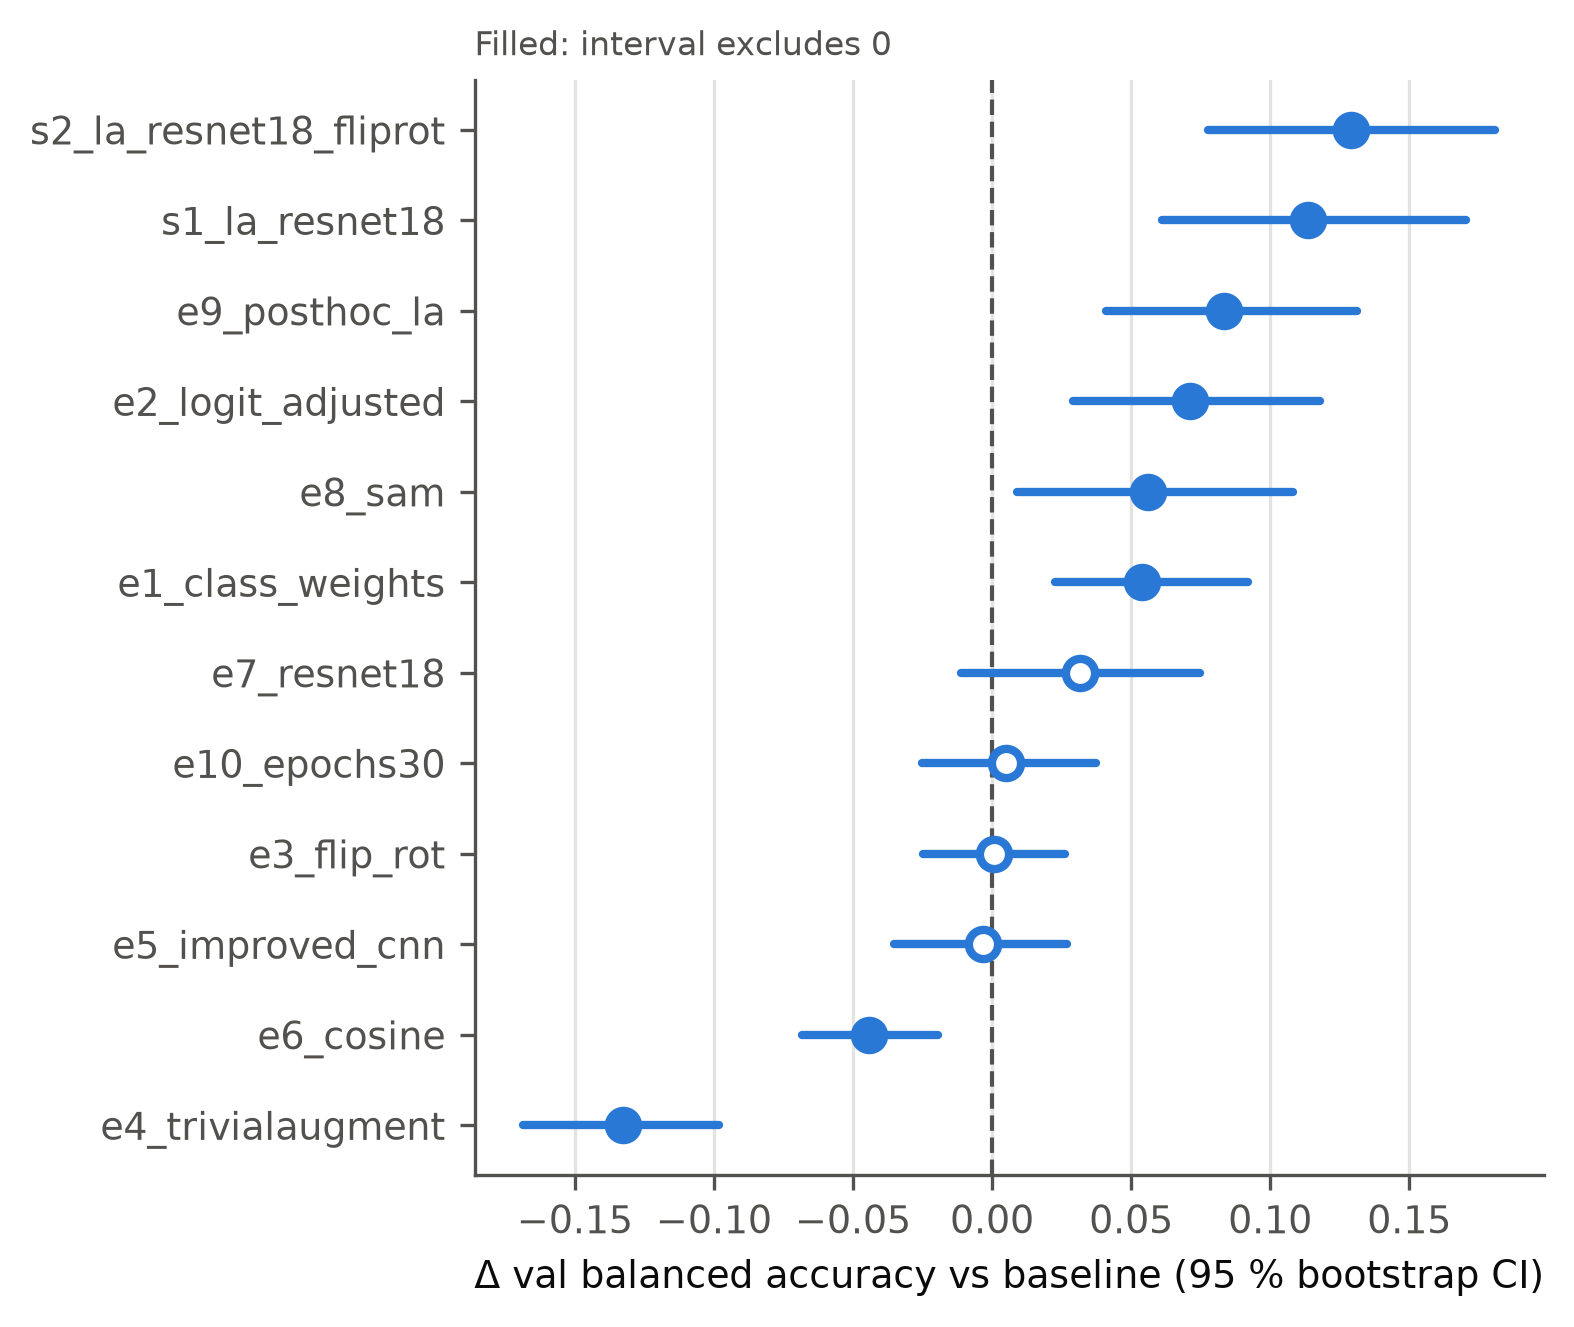
\includegraphics[width=\columnwidth]{figures/forest_delta.png}
\caption{Difference in validation balanced accuracy to the baseline with 95\,\% bootstrap interval (filled:
interval excludes 0).}
\label{fig:forest}
\end{figure}

Table~\ref{tab:test} gives the single test evaluation. The final model improves balanced accuracy by 0.184
[+0.136, +0.232]. Dermatofibroma sensitivity rises from 0.09 to 0.57, melanoma from 0.34 to 0.64 and vascular
lesions from 0.45 to 0.93, while nevus sensitivity falls from 0.91 to 0.73; macro-F1 changes little (0.479 to
0.500). Fig.~\ref{fig:sens} shows the same pattern on the validation set.

\begin{table*}[t]
\caption{Test set, evaluated once after the freeze: both models are 3-seed ensembles. Per-class columns are
sensitivities; $\Delta$ is a paired bootstrap on the 2\,005 test images}
\label{tab:test}
\centering
\begin{tabular}{lcccccccccc}
\toprule
model & bal.\ acc. & $\Delta$ [95\,\% CI] & macro-F1 & akiec & bcc & bkl & df & mel & nv & vasc \\
\midrule
baseline & 0.448 & -- & 0.479 & 0.33 & 0.55 & 0.46 & 0.09 & 0.34 & 0.91 & 0.45 \\
final & \textbf{0.632} & +0.184 [+0.136, +0.232] & 0.500 & 0.52 & 0.50 & 0.55 & 0.57 & 0.64 & 0.73 & 0.93 \\
\bottomrule
\end{tabular}
\end{table*}

\begin{figure}[t]
\centering
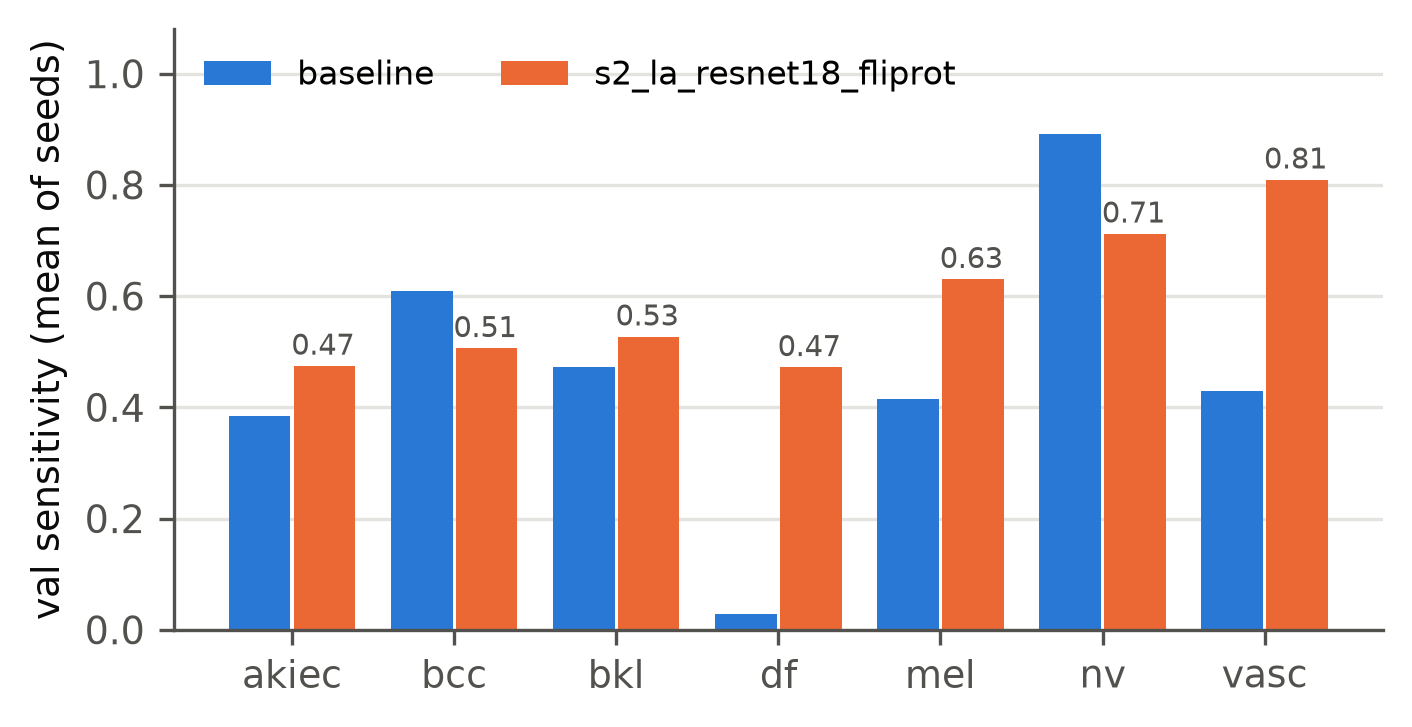
\includegraphics[width=\columnwidth]{figures/sensitivity.png}
\caption{Validation sensitivity per class (mean over seeds): baseline vs.\ S2.}
\label{fig:sens}
\end{figure}

\begin{figure}[t]
\centering
\IfFileExists{figures/tensorboard.png}{%
\includegraphics[width=\columnwidth]{figures/tensorboard.png}}{%
\fbox{\parbox[c][3cm][c]{0.9\columnwidth}{\centering TODO: TensorBoard screenshot\\
(\texttt{figures/tensorboard.png})}}}
\caption{Validation balanced accuracy per epoch for all runs in TensorBoard.}
\label{fig:tb}
\end{figure}

\section{Discussion}
\textbf{What worked.} Every change that corrects the imbalance helped, as expected for a metric that weights
the 80 dermatofibroma images like the 4\,693 nevi. Logit adjustment did slightly better than class weights,
consistent with its consistency for the balanced error~\cite{menon2021logit}. The pretrained ResNet alone was
not a clear gain, but with the logit-adjusted loss it gave the largest step: it kept nevus sensitivity at
0.76 (E2 alone: 0.58), so the imbalance correction over-corrected less and macro-F1 recovered (0.509 vs.\
0.400). Averaging the three seed models added about two points.

\textbf{What did not.} TrivialAugment and the cosine schedule were clearly worse within the fixed 10-epoch
budget. A likely reason for TrivialAugment is that strong augmentation needs more epochs; we did not test longer
budgets for E4 or E6, so both explanations are hypotheses. Training three times longer (E10) did not help the
small CNN, so training time is not what limits it; a larger plain CNN (E5) did not help either and was unstable
across seeds (std 0.047). SAM added nothing on top of E2.

\textbf{Trade-off and uncertainty.} The gain in balanced accuracy is bought with lower nevus sensitivity
(0.91 to 0.73 on test): more harmless moles are flagged. Benign keratosis, actinic keratoses and basal cell
carcinoma stay near 0.5. With 12--33 validation images in three classes, intervals are wide, and with this
many comparisons a few intervals may exclude zero by chance; the stacking steps over E2 are not individually
significant. The test score (0.632) is above the validation score (0.609), within this noise.

\textbf{Limitations and next steps.} 28$\times$28 inputs, one dataset, possible same-lesion images across
splits, and a fixed 10-epoch budget for every variant. Next we would tune $\tau$ and the epoch budget for the
ResNet, try deferred re-weighting, and use the higher-resolution MedMNIST+ images~\cite{doerrich2025medmnistplus}.

\section{Conclusion}
A logit-adjusted loss is the most effective single change for balanced accuracy on DermaMNIST, and it works
best together with a pretrained ResNet-18 on upsampled inputs. Our final three-seed ensemble raises test
balanced accuracy from 0.448 to 0.632, mainly by finding dermatofibroma, melanoma and vascular lesions, at
the cost of nevus sensitivity.

\section*{AI use statement}
% TODO (team): rewrite in your own words; keep only checks you have actually done.
We used Claude (Anthropic) through Claude Code throughout the project: it wrote most of the training,
evaluation, export and app code, ran the experiments on our laptop, made the figures, and drafted the README
and this report. [TODO: what the team reviewed in the code.] [TODO: confirm that the numbers were compared
with \texttt{results/summary.csv} and \texttt{results/test/}.] [TODO: confirm that every reference was checked
against the original paper.]

\section*{Contribution statement}
% TODO (team): who did what, 2-3 sentences.
TODO.

\bibliographystyle{IEEEtran}
\bibliography{references}

\end{document}
